%% stallings.tex - Stallings folding algorithm is P-complete
%%
%% Copyright 2012, 2013, 2014 Jeffrey Finkelstein.
%%
%% This LaTeX markup document is made available under the terms of the Creative
%% Commons Attribution-ShareAlike 4.0 International License,
%% https://creativecommons.org/licenses/by-sa/4.0/.
\documentclass{article}

\usepackage{amsmath}
\usepackage{amssymb}
%% This must come before hyperref.
\usepackage{amsthm}
%% This is strongly recommended by biblatex.
\usepackage[english]{babel}
\usepackage[backend=biber]{biblatex}
\usepackage[T1]{fontenc}
%% This must come before csquotes.
\usepackage[utf8]{inputenc}
\usepackage{lmodern}
%% This is strongly recommended by biblatex.
\usepackage{csquotes}
%% This must come before hyperref.
\usepackage{thmtools}
%% This must come before complexity.
\usepackage{hyperref}
\usepackage{complexity}
\usepackage[firstpage]{draftwatermark}
\usepackage{microtype}
\usepackage{textcomp}
\usepackage{tikz}
\usepackage{tkz-graph}

\LoadMicrotypeFile{cmr}
\SetProtrusion
    [load=lmr-T1]
    {encoding=T1, family=lmr}
    {
      \textquotedblright = {,1000},
      \textquotedblleft = {1000,},
      {'} = {,1000},
      {,} = {,1000},
      {:} = {,1000},
      {;} = {,1000},
      {.} = {,1000}
    }

%% Set the ``work-in-progress'' watermark for the first page.
\SetWatermarkLightness{0.9}
\SetWatermarkText{Work-in-progress}
\SetWatermarkFontSize{3.5cm}

%% Set the title and author of the PDF file.
\hypersetup{pdftitle={Stallings' Folding Process is Inherently Sequential}, pdfauthor={Jeffrey Finkelstein}}

%% Declare the bibliography file.
\addbibresource{stallings.bib}

%% Declare theorem-like environments.
\declaretheorem[numberwithin=section]{theorem}
\declaretheorem[numberlike=theorem]{corollary}
\declaretheorem[numberlike=theorem]{conjecture}
\declaretheorem[numberlike=theorem]{lemma}
\declaretheorem[numberlike=theorem, style=definition]{definition}
\declaretheorem[numberlike=theorem, style=definition]{todo}

%% Custom commands are declared here.
\newcommand{\email}[1]{\textlangle\href{mailto:#1}{\nolinkurl{#1}}\textrangle}
%\newcommand{\todo}[1]{\textbf{TODO #1}}
\newcommand{\FGR}{\textsc{Free Group Rank}}
\newcommand{\FD}{\textsc{Folded Density}}
\newcommand{\Flow}{\textsc{Flow($F$)}}
\newcommand{\BS}{\textsc{Bitwise Stallings}}
\newcommand{\NDM}{\textsc{Centered NFA-to-DFA Minimization}}
\newcommand{\PFolds}{\textsc{Parallel Folds}}
\newcommand{\gen}[1]{\langle #1 \rangle}
\newcommand{\Core}{\textnormal{Core}}
\DeclareMathOperator{\pos}{pos}
\newcommand{\nega}{\textnormal{neg}}
\newcommand{\Spm}{S^{\pm1}}

%% Redefine the footnote environment so it has no reference and no number.
\long\def\symbolfootnote#1{\begingroup%
\def\thefootnote{\fnsymbol{footnote}}\footnotetext{#1}\endgroup}

%% Define the author, title, and date for the document.
\author{Jeffrey~Finkelstein\\ Computer Science Department, Boston University}
\title{Stallings' Folding Process is Inherently Sequential}

\begin{document}

\maketitle

\symbolfootnote{%
  Copyright 2012, 2013, 2014 Jeffrey~Finkelstein \email{jeffreyf@bu.edu}.

  This document is licensed under the Creative Commons Attribution-ShareAlike 4.0 International License, which is available at \mbox{\url{https://creativecommons.org/licenses/by-sa/4.0/}}.
  The \LaTeX{} markup that generated this document can be downloaded from its website at \mbox{\url{https://github.com/jfinkels/document}}.
  The markup is distributed under the same license.
}

\section{Introduction}
% Foreword

% context (focus on anyone) why now? - current situation, and why the need is so important
The problem of computing the minimum rank of a finitely generated subgroup of a free group is inherently sequential---that is, allowing many processors to work together in parallel offers no significant speedup when solving the problem.
%Inherently sequential computational problems have efficient algorithms but do not have highly parallel algorithms, unless $\P = \NC$ (an equality considered unlikely).
One way of computing the minimum rank of the subgroup is by computing the size of a Nielsen reduced set equivalent to the generating set of the subgroup.
% need (focus on readers) why you? - why this is relevant to the reader, and why something needed to be done
Although it is computable in polynomial time, the Nielsen reduction is relatively complicated and the polynomial is of relatively large degree.
A more efficient solution is to instead reduce the problem to a more easily solved graph problem; a finitely generated subgroup of a free group has a very natural representation as a directed, labeled graph.
Stallings' process for ``folding'' a directed labeled graph \cite[Algorithm~5.4]{stallings83} is an analog of the Nielsen reduction for computing a minimal generating set for a free group.
%%% relevant existing work, given as part of the need
% task (focus on author) why me? - what was undertaken to address the need
Can Stallings' folding process solve the problem of finding the rank of a subgroup more quickly than the Nielsen reduction can?
% object (focus on document) why this document - what the document covers
This paper proves that it cannot by showing that some computational problems concerning the execution of this process are inherently sequential.

% Summary
%
% findings (focus on author) what? - what the work revealed when performing the task
We show that computing a certain measure of density on the graph produced by Stallings' folding process is inherently sequential.
We also show that counting the number of redundant steps in the process is inherently sequential.
Finally, although we are unable to show that Stallings' folding process is inherently sequential according to the definition of an ``inherently sequential algorithm'', we do show that the function is $\FP$-complete.
% conclusion (focus on readers) so what? - what the findings mean for the audience
We conclude that asymptotically Stallings' folding process does not benefit from added parallelism.
% perspective (focus on anyone) what now? - what should be done next
We stop short of determining if Stallings' folding process admits a highly parallel approximation algorithm.
This is important for developing a thorough understanding of the computational complexity of this mathematical algorithm: a highly parallel approximation for Stallings' folding process may yield a highly parallel approximation for the rank of a free group, which has applications in computational algebra systems.

\section{Preliminaries}

\subsection{Languages and strings}

A finite set $\Sigma$ is called an \emph{alphabet}.
If $\Sigma$ is an alphabet, a \emph{word} over $\Sigma$ is a finite sequence of symbols from $\Sigma$.
The set of all words over $\Sigma$ is denoted $\Sigma^*$.
If $w$ is a word, the \emph{length} of $w$, denoted $|w|$, is the length of its underlying sequence.
A \emph{language} is a subset of $\Sigma^*$.

\subsection{Computational complexity}

We assume some familiarity with two well-known models of computation: the Turing machine and the random access machine (RAM).
For definitions and background information on these models, see \autocite{savage98}.

We say a Turing machine $M$ \emph{decides} a language $L$ in polynomial time if for all words $x$ in $\Sigma^*$, we have $x \in L$ if and only if $M$ accepts $x$, and $M$ halts within time $p(|x|)$ for some polynomial $p$.
A function $f$ is \emph{computable} if there is a Turing machine that, on any input $x$, always halts with $f(x)$ on its tape.
The complexity class $\P$ is the class of all languages that can be decided in polynomial time.
The complexity class $\FP$ is the collection of functions that are computable by a Turing machine in polynomial time (that is, there is a Turing machine $M$ and a polynomial $p$ such that on inputs $x$ of length $n$, the machine $M$ halts with $f(x)$ on its tape within $p(n)$ steps).
The complexity class $\L$ is the class of all languages that can be decided on a Turing machine with a read-only input tape and a read-write work tape using at most $O(\log n)$ space on the work tape.
The complexity class $\FL$ is the collection of functions that are computable on a Turing machine with a read-only input tape, a write-only output tape, and a read-write work tape using at most $O(\log n)$ space on the work tape.

If $L$ is a language, let $L(w)$ denote the \emph{characteristic function} of $w$, defined by $L(w) = 1$ if $w \in L$ and $L(w) = 0$ if $w \notin L$.
If $L_1$ and $L_2$ are languages, there is a \emph{logarithmic space many-one reduction} from $L_1$ to $L_2$ if there is a function $f \in \FL$ such that $x \in L_1$ if and only if $f(x) \in L_2$.
There is a \emph{logarithmic space nonadaptive Turing reduction} from $L_1$ to $L_2$ if there is a Turing machine $M$ and a function $h \in \FL$ such that $x \in L_1$ if and only if $M(x, L_2(y_1), \dotsc, L_2(y_t))$ accepts, where $(y_1, \dotsc, y_t)$ is the output of $h(x)$.
If $L$ is a language and $F$ is a computable function, there is a \emph{logarithmic space Turing reduction} from $L$ to $F$ if there is an oracle Turing machine $M$ such that $x \in L$ if and only if $M^F(x)$ accepts.
If furthermore $M$ makes at most one query to $F$, the reduction is called a \emph{logarithmic space single query Turing reduction}.

Let $L$ be a language and $F$ be a computable function.
If there is a logarithmic space many-one reduction from each language in $\P$ to $L$, then $L$ is \emph{$\P$-hard}; if furthermore $L$ is in $\P$, then $L$ is \emph{$\P$-complete}.
Languages that are $\P$-complete are considered ``inherently sequential'', because a highly parallel algorithm for any one of them would imply a highly parallel algorithm for each language in $\P$, a result considered unlikely.
If there is a logarithmic space Turing reduction from each language in $\P$ to $F$, then $F$ is \emph{$\FP$-hard}; if furthermore $F$ is in $\FP$, then $F$ is \emph{$\FP$-complete}.

\subsection{Free groups}

If $S$ is an alphabet, we define the set of \emph{formal inverses} for $S$, denoted $S^{-1}$, by $\{ s^{-1} \,|\, s \in S \}$.
In this case, the symbol $s^{-1}$ is the formal inverse of $s$ and vice versa.
Let $\Spm$ denote the set $S \cup S^{-1}$.
A word $w$ of length $n$ over $\Spm$ can be written as $s_1s_2\cdots s_n$ where $s_i \in \Spm$ for each $i \in \{1, \dotsc, n\}$.
If $u$ and $v$ are words over $\Spm$, where $u = u_1 u_2 \dotsb u_n$ and $v = v_1 v_2 \dotsb v_m$, then the \emph{concatenation} of $u$ and $v$, denoted $u \circ v$ or simply $uv$, is the word $u_1 u_2 \cdots u_n v_1 v_2 \cdots v_m$.
A word is \emph{freely reduced} if it contains no two adjacent symbols that are inverses.
The \emph{free group} on $S$ is the set of freely reduced words on $\Spm$ under the operation which concatenates two words then freely reduces the result.
In this free group, a word $w$ where $w = w_1 w_2 \cdots w_{i - 1} s s^{-1} w_{i + 2} \cdots w_n$ (which is not freely reduced) is equivalent to the freely reduced word $w' = w_1 w_2 \cdots w_{i - 1} w_{i + 2} \cdots w_n$.
Each word over $\Spm$ has a unique, freely reduced representation (see for example, \cite[Section~I.1]{ls77}).
We denote this freely reduced representative of the word $w$ by $\rho(w)$.
If $A$ is a set of words, we define $\rho(A)$ by $\rho(A) = \{ \rho(a) \, | \, a \in A\}$.
A \emph{finitely generated subgroup} of the free group on $S$ is the closure of a finite set of words over $\Spm$ under the free group operation.
If $U$ is a finite set of words, the subgroup generated by $U$ is denoted $\gen{U}$.
The \emph{rank} of a finitely generated subgroup is the cardinality of a generating set of minimum size.

\subsection{Graphs}

A two-tuple $(V, E)$ is a \emph{directed graph} if $V$ is a set of vertices and $E$ is a multiset of elements from $V \times V$.
In this work, we write ``directed graph'' instead of ``directed multigraph''; note that multiple, parallel edges are allowed.
We also refer to the ``edge set'' of a directed graph when we mean ``edge multiset''.
If $G$ is a directed graph, we denote the vertex set of $G$ by $V(G)$ and the edge set of $G$ by $E(G)$.
If $e$ is an edge in a graph and $e = (u, v)$, where $u$ and $v$ are vertices, then the \emph{origin} of $e$, denoted $o(e)$, is defined by $o(e) = u$ and the \emph{terminus} of $e$, denoted $t(e)$, is defined by $t(e) = v$.
Two edges (in a multigraph) are \emph{parallel} if they have the same origin and terminus.
A \emph{path from $u$ to $v$} in $G$, or more simply, a \emph{path}, is a finite sequence of edges, $(e_1, e_2, \dotsc, e_n)$, such that $o(e_1) = u$, $t(e_n) = v$, and $t(e_i) = o(e_{i + 1})$ for all $i \in \{1, \dotsc, n - 1\}$.
A \emph{rooted circle} is a path from ``root'' vertex $v \in V(G)$ to the same vertex, along which each intermediate vertex, except possibly $v$, is incident to exactly two edges (namely, the one preceding it in the path and the one following it in the path).
The directed graph $G$ is a \emph{flower graph} with respect to a vertex $v \in V(G)$ if it equals the union of circles rooted at $v$.
%% TODO better definitions of minimal spanning trees
If $G$ is a directed graph, a \emph{tree} $T$ with root $v$ is an acyclic subgraph of $G$ in which there is a path in $T$ from $v$ to every vertex in $V(T)$.
A tree $T$ with root $v$ is a \emph{spanning tree} for $G$ if there is a path in $T$ from $v$ to every vertex in $V(G)$.
A spanning tree is \emph{minimal} if no edges can be removed without violating the spanning property.
The \emph{additive density} of $G$, denoted $\delta(G)$, is defined by $\delta(G) = |E(G)| - |V(G)|$ for all graphs $G$.

We say $G$ is \emph{labeled} by $S$ if there exists a function $\mu \colon E(G) \to S$.
If $G$ is a labeled, directed graph, then its \emph{inverse graph}, denoted $\hat{G}$, has the same vertex set and edge set, but wherever there is an edge $(u, v) \in E(G)$ with label $s$ we add the inverse edge $(v, u)$ to $E(\hat{G})$ with label $s^{-1}$.
The \emph{positive} edges of $\hat{G}$ are the edges with labels in $S$ and the \emph{negative} edges are those with labels in $S^{-1}$.
If $E$ is a set of directed, labeled edges, we denote the positive edges in $E$ by $\pos(E)$ and the negative edges by $\nega(E)$.
The \emph{label} of a path $p$, denoted $\mu(p)$, is the sequence of labels of each of its constituent edges.
We sometimes abuse notation for the sake of convenience and discuss a path in $G$ when what we mean is a path in the subgraph induced by the positive edges of $\hat{G}$ in which edges $e$ with the inverse orientation are allowed, but their labels $\mu(e)$ are read as the corresponding inverse label $\mu(e)^{-1}$.
Analogous to freely reduced words in the free group on $S$, a \emph{reduced path} in $G$ is a path which does not contain any adjacent pairs of edges such that their labels are inverses.

\subsection{Languages of labeled graphs}

If $G$ is a directed graph labeled by $S$ and $v \in V(G)$, then the \emph{language of $G$ with respect to $v$}, denoted $L(G, v)$, is defined by
\begin{equation*}
  L(G, v) = \{ \mu(p) \, | \, p \text{ is a reduced path in } G \text{ from } v \text{ to } v\}.
\end{equation*}
The \emph{reduced language}, denoted $\rho(L(G, v))$, is defined by $\rho(L(G, v)) = \{ \rho(w) \, | \, w \in L(G, v) \}$.
The \emph{core} of a labeled, directed graph $G$ with respect to a vertex $v \in V(G)$, denoted $\Core(G, v)$, is the subgraph of $G$ induced by the set of all edges which are in some reduced path from $v$ to $v$.
A labeled, directed graph $G$ is a \emph{core graph} with respect to a vertex $v \in V(G)$ if $\Core(G, v) = G$.
A pair of edges is \emph{foldable} if they have the same label and they share an origin or a terminus.
A directed graph $G$ labeled by $S$ is \emph{folded} if there are no foldable edges.
In other words, for each vertex $v \in V(G)$ and each symbol $s \in S$, there is at most one edge in $E(G)$ with origin $v$ and label $s$ and there is at most one edge in $E(G)$ with terminus $v$ and label $s$.
Stated another way, $G$ is folded if there is no vertex $v \in V(G)$ such that $v$ has two (or more) in-edges with the same label or two (or more) out-edges with the same label.
Informally, a \emph{fold} is a function which identifies not only two foldable edges but also the vertex opposite from their shared incident vertex.
%% TODO state that every graph has a folded representative, F(G) that produces
%% the same freely reduced language
\emph{Stallings' folding process}, defined in \autocite[Algorithm~5.4]{stallings83}, is a function, denoted $F$, that operates on labeled, directed graphs.
It proceeds by repeatedly choosing a foldable pair of edges (say, the lexicographically first pair) and folding them until there are no more foldable edges.

\begin{theorem}[{\autocite{touikan06}}]\label{thm:finfp}
  Stallings' folding process, $F$, is in $\FP$.
\end{theorem}

The input to $F$ is a finite alphabet $S$, a directed graph $G$, and a label function $\mu \colon E(G) \to S$.
The output of $F$ is the same alphabet $S$, a directed graph $G'$, and a label function $\mu' \colon E(G') \to S$.
For the sake of brevity, instead of writing $(S, G', \mu') = F(S, G, \mu)$, we will write $G' = F(G)$, when the alphabet and the label function are clear from context.

% TODO Move these definitions into the results section?
\subsection{Computational problems}

We will utilize the following computational problems.

\begin{definition}[\FGR]
  \mbox{} \\
  \begin{tabular}{r p{9.5cm}}
    \textbf{Instance:} & finite alphabet $S$, finite set $U$ of freely reduced words over $\Spm$, positive integer $k$. \\
    \textbf{Question:} & Does $\gen{U}$ in the free group on $S$ have rank $k$ or less?
  \end{tabular}
\end{definition}

(\FGR{} should be thought of as a minimization problem, but is defined as a decision problem in order to facilitate proofs of hardness).
\FGR{} is \P-complete \cite[Theorem~4.9]{am84} (see also \cite[Problem~A.8.11]{ghr95}).
In fact, the algorithm that shows that this problem is decidable in polynomial time is constructive; not only does it compute the rank of $\gen{U}$, it does so by also computing a set $V$ such that $V$ is Nielsen reduced and $\gen{U} = \gen{V}$.
We will use this fact to show the $\P$-completeness of some related problems, and ultimately Stallings' folding process itself.

\begin{definition}[\FD]
  \mbox{} \\
  \begin{tabular}{r p{9.5cm}}
    \textbf{Instance:} & finite alphabet $S$, directed graph $G$, label function $\mu \colon E \to S$, integer $k$. \\
    \textbf{Question:} & Does $F(G)$ have additive density at most $k$?
  \end{tabular}
\end{definition}

\begin{definition}[\PFolds]
  \mbox{} \\
  \begin{tabular}{r p{9.5cm}}
    \textbf{Instance:} & finite alphabet $S$, directed graph $G$, label function $\mu \colon E \to S$, integer $k$. \\
    \textbf{Question:} & Is $N^\|_F(G)$ greater than or equal to $k$? Here, $N^\|_F(G)$ is the number of folds produced by running $F$ on input $G$ that are folds of a pair of parallel edges.
  \end{tabular}
\end{definition}

Suppose $M$ is an arbitary RAM.
For any input $x$, each statement executed by $M$ when run on input $x$ has an associated \emph{value}.
For example, the value of an ``add'' instruction is the integer that results from the addition and the value of a ``write'' instruction is the integer written to memory.
The \emph{flow function} of $M$, denoted $f_M$, is defined by $f_M(x, t) = ((1, v_1), \dotsc, (t, v_t))$, where $v_i$ is the value associated with statement $i$ in the execution of $M$ on input $x$.
Define $f_M(x)$ by $f_M(x) = f_M(x, T(|x|))$, where $T(n)$ is the function bounding the maximum running time of $M$ on inputs of length $n$.

\begin{definition}[\textsc{Flow($M$)}]
  \mbox{} \\
  \begin{tabular}{r p{9.5cm}}
    \textbf{Instance:} & binary string $x$, positive binary integer $i$, bit $j$. \\
    %% \textbf{Instance:} & finite alphabet $S$, directed graph $G$, label function $\mu \colon E \to S$, positive binary integer $i$, bit $j$. \\
    \textbf{Question:} & Does the $i$th bit of $f_M(x)$ equal $j$?
  \end{tabular}
\end{definition}

We say the function computed by $M$ is \emph{inherently sequential} if \textsc{Flow($M$)} is $\P$-complete (\autocite[Definition~8.2.2]{ghr95}).

\section{Transforming a subgroup into a graph}
% Foreword

% context (focus on anyone) why now? - current situation, and why the need is so important
How can a simple graph algorithm be used to compute the rank of a finitely generated subgroup of a free group?
% need (focus on readers) why you? - why this is relevant to the reader, and why something needed to be done
First we need to prove that for each set of generators there is an ``equivalent'' graph that has the properties we desire.
% task (focus on author) why me? - what was undertaken to address the need
We restate a result implicit in \autocite{km02} so that we can use this equivalence in a complexity theoretic proof.
% object (focus on document) why this document - what the document covers
\autoref{lem:main} is a summary and restatement of some results in \autocite{km02}; please see the referenced lemmas and propositions for more information and complete proofs.

% Summary
%
% findings (focus on author) what? - what the work revealed when performing the task
According to the following lemma, each finitely generated subgroup of a free group can be represented as a flower graph whose ``petals'' are labeled with the words in the generating set.
In this way, a word in the generating set corresponds to a cycle that begins at the root, proceeds around a petal, and terminates at the root.
Concatenation of words then corresponds to a walk consisting of a concatenation of cycles, always returning to the root.
% conclusion (focus on readers) so what? - what the findings mean for the audience
Since this transformation from group to graph is efficiently computable, it allows to translate statements about labeled directed graphs to statements about free groups.
% perspective (focus on anyone) what now? - what should be done next
With this transformation and the fact that \FGR{} is $\P$-complete, we can show that the graph theoretic problems concerning Stallings' folding process are $\P$-complete as well.

\begin{lemma}\label{lem:main}
  For each finite alphabet $S$ and finite set $U$ of freely reduced words over $\Spm$, there is a graph $G$ and a label function $\mu \colon E(G) \to S$ such that
  \begin{enumerate}
  \item $G$ and $\mu$ are computable in logarithmic space with respect to the size of $S$ and $U$,
  \item $G$ is a flower graph and a core graph (with respect to the same vertex),
  \item there is a set $Y$ of words induced by paths in $F(G)$ such that
    \begin{itemize}
    \item the rank of $\gen{U}$ equals $|Y|$,
    \item $|Y|$ is computable in logarithmic space with respect to the size of $F(G)$.
    \end{itemize}
  \end{enumerate}
\end{lemma}
\begin{proof}
  Suppose $U$ is a finite set of words $\{u_1, u_2, \dotsc, u_m\}$ and for each $i \in \{1, \dotsc, m\}$ we have $u_i = u_{i, 1}u_{i, 2}\dotsb u_{i, n_i}$ where $n_i$ is the length of $u_i$.
  Construct the directed graph $G$ as follows.
  Create a vertex $v_0$, which will be the ``root'' of the flower.
  Create one circle rooted at $v_0$ for each word $u$ in $U$, and each circle is divided into $|u|$ edges, one for each symbol of $u$.
  Each edge of the circle is then labeled with the corresponding symbol in $u$.
  Wherever the graph contains a label $s^{-1}$, the inverse of a symbol $s$ in $S$, that edge is reversed (that is, $(v, w)$ is replaced with $(w, v)$) and we replace the label $s^{-1}$ with the label $s$ on the reversed edge.
  In this way we have constructed a graph with only positive edges; this simplifies our proof a bit.

  This function is computable in logarithmic space because a loop over the set $U$ requires $O(\log |U|)$ space, a loop over a word $u \in U$ requires $O(\log |u|)$ space, and writing the adjacency matrix of the graph and the corresponding labels can be done in constant space.
  Thus, item 1 is satisfied.

  Since it is the union of circles rooted at $v_0$, the graph $G$ is a flower graph with respect to $v_0$.
  Since each circle corresponds to a word in $U$, and each word in $U$ is freely reduced, $G$ is also a core graph with respect to $v_0$.
  Thus, item 2 is satisfied

  Now in order to construct $Y$, we examine the properties of the graph $G$ under $F$, Stalling's folding process.
  Let $G' = F(G)$ and $v'_0$ be the image of $v_0$ under the sequence of foldings produced by $F$ on input $G$.
  We know $G'$ has a spanning tree $T$ which is geodesic with respect to $v'_0$ by \cite[Lemma~6.6]{km02}.
  For any vertex $z$ in $V(G')$, let $[v'_0, z]_T$ denote the path from $v'_0$ to $z$ within the spanning tree $T$.
  For each edge $e$ in $E(G') \setminus E(T)$ (in other words, $e$ is an edge in $G'$ not in the spanning tree $T$), let $p_e$ denote the path that results from the concatenation of the three paths $[v'_0, o(e)]_T, e, [t(e), v'_0]_T$.
  (Since $T$ is a spanning tree, $[v'_0, o(e)]_T$ and $[t(e), v'_0]_T$ must exist.)
  Define the set of words $Y$ as
  \begin{equation*}
    Y = \left\{\mu(p_e) \, \middle| \, e \in E(G') \setminus E(T) \right\}.
  \end{equation*}
  Now
  \begin{align*}
    \gen{U} & = \rho(L(G, v_0)) & \qquad \text{ (by \cite[Proposition~3.8]{km02})} \\
            & = \rho(L(G', v'_0)) & \qquad \text{ (by \cite[Lemma~3.4]{km02})} \\
            & = L(G', v'_0), & \qquad \text{ (by \cite[Lemma~2.9]{km02})} \\
            & = \gen{Y}, & \qquad \text{ (by \cite[Lemma~6.1]{km02})}
  \end{align*}
  Since, $\gen{U} = \gen{Y}$, their ranks are equal.
  Finally, the rank of $\gen{Y}$ is $|Y|$, since $Y$ is Nielsen reduced by \cite[Proposition~6.7]{km02}.
  Therefore, the rank of $\gen{U}$ equals $|Y|$.

  Computing $|Y|$ can be done by counting the number of (positive) edges in $G'$ not in $T$.
  Computing $T$ from $G'$ can be done recursively in logarithmic space (by recursively computing $T_n$, the geodesic spanning tree for all vertices at distance $n$ from $v_0$; this requires $O(n)$ levels of recursion, each of which requires looping over $O(n^2)$ edges and checking if each edge is adjacent to one already in the spanning tree from the next level of recursion, thereby requiring at most $O(\log n)$ space).
\end{proof}

%% The figure illustrating an example run of Stallings' folding process is
%% inserted here.
%\begin{figure}
  \caption{\label{fig:example}%
    An step-by-step execution of Stallings' folding process on the graph corresponding to the set of words $U$ defined by $U = \{aab, aba^{-1}, ba^{-1}ba\}$ (this example is from \autocite[Figure~4]{km02}).
  Each picture shows in orange the pair of edges to be folded.}
  \begin{center}
    \begin{tabular}{c c}
      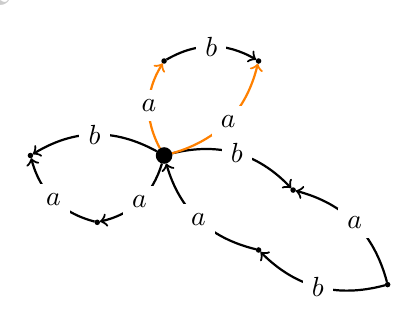
\begin{tikzpicture}[->]
        \GraphInit[vstyle=Simple]
        \SetGraphUnit{1.2}
        \tikzset{VertexStyle/.style={shape=circle, fill=black,
            minimum size=2pt, inner sep=0pt}}
        \tikzset{EdgeStyle/.style={bend left}}

        \begin{scope}[rotate={45}]
          \begin{scope}[VertexStyle/.append style = {minimum size=6pt}]
            \Vertex{v0}
          \end{scope}
          \WE(v0){a}
          \NO(a){b}
        \end{scope}

        \Edge[label={$a$}](v0)(a)
        \Edge[label={$a$}](a)(b)
        \Edge[label={$b$}, style={<-}](b)(v0)

        \begin{scope}[rotate=30]
          \SOEA(v0){c}
        \end{scope}
        \SOEA(c){d}
        \begin{scope}[rotate=30]
          \NOWE(d){e}
        \end{scope}

        \Edge[label={$b$}](v0)(c)
        \Edge[label={$a$}, style={<-}](c)(d)
        \Edge[label={$b$}](d)(e)
        \Edge[label={$a$}](e)(v0)

        \NO(v0){f}
        \EA(f){g}

        \Edge[color=orange, label={$a$}](v0)(f)
        \Edge[label={$b$}](f)(g)
        \Edge[color=orange, label={$a$}, style={<-}](g)(v0)
      \end{tikzpicture}
      &
      %% Picture 2
      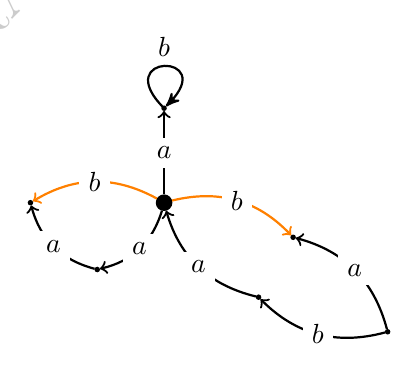
\begin{tikzpicture}[->]
        \GraphInit[vstyle=Simple]
        \SetGraphUnit{1.2}
        \tikzset{VertexStyle/.style={shape=circle, fill=black,
            minimum size=2pt, inner sep=0pt}}
        \tikzset{EdgeStyle/.style={bend left}}

        \begin{scope}[rotate={45}]
          \begin{scope}[VertexStyle/.append style = {minimum size=6pt}]
            \Vertex{v0}
          \end{scope}
          \WE(v0){a}
          \NO(a){b}
        \end{scope}

        \Edge[label={$a$}](v0)(a)
        \Edge[label={$a$}](a)(b)
        \Edge[color=orange, label={$b$}, style={<-}](b)(v0)

        \begin{scope}[rotate=30]
          \SOEA(v0){c}
        \end{scope}
        \SOEA(c){d}
        \begin{scope}[rotate=30]
          \NOWE(d){e}
        \end{scope}

        \Edge[color=orange, label={$b$}](v0)(c)
        \Edge[label={$a$}, style={<-}](c)(d)
        \Edge[label={$b$}](d)(e)
        \Edge[label={$a$}](e)(v0)

        \NO(v0){f}

        \Edge[label={$a$}, style={bend left=0}](v0)(f)
        % {labelstyle=above} is needed here because tkz-graph seems to refuse to
        % add the appropriate whitespace around the label.
        \Loop[label={$b$}, dir=EA, dist=1cm, labelstyle={above}](f)
      \end{tikzpicture}
      \\
      %% Picture 3
      \begin{tikzpicture}[->]
        \GraphInit[vstyle=Simple]
        \SetGraphUnit{1.2}
        \tikzset{VertexStyle/.style={shape=circle, fill=black,
            minimum size=2pt, inner sep=0pt}}
        \tikzset{EdgeStyle/.style={bend left}}

        \begin{scope}[VertexStyle/.append style = {minimum size=6pt}]
          \Vertex{v0}
        \end{scope}
        \NOEA(v0){a}

        \Edge[color=orange, label={$a$}](v0)(a)
        \Edge[label={$a$}](a)(c)

        \begin{scope}[rotate=30]
          \SOEA(v0){c}
        \end{scope}
        \SOEA(c){d}
        \begin{scope}[rotate=30]
          \NOWE(d){e}
        \end{scope}

        \Edge[label={$b$}](v0)(c)
        \Edge[label={$a$}, style={<-}](c)(d)
        \Edge[label={$b$}](d)(e)
        \Edge[label={$a$}](e)(v0)

        \SOWE(v0){f}

        \Edge[color=orange, label={$a$}, style={bend left=0}](v0)(f)
        % {labelstyle=below left} is needed here because tkz-graph seems to
        % refuse to add the appropriate whitespace around the label.
        \Loop[label={$b$}, dir=NOWE, dist=1cm, labelstyle={below left}](f)
      \end{tikzpicture}
      &
      %% Picture 4
      \begin{tikzpicture}[->]
        \GraphInit[vstyle=Simple]
        \SetGraphUnit{1.2}
        \tikzset{VertexStyle/.style={shape=circle, fill=black,
            minimum size=2pt, inner sep=0pt}}
        \tikzset{EdgeStyle/.style={bend left}}

        \begin{scope}[VertexStyle/.append style = {minimum size=6pt}]
          \Vertex{v0}
        \end{scope}
        \NOEA(v0){a}

        \Edge[label={$a$}](v0)(a)
        \Edge[color=orange, label={$a$}](a)(c)

        \begin{scope}[rotate=30]
          \SOEA(v0){c}
        \end{scope}
        \SOEA(c){d}
        \begin{scope}[rotate=30]
          \NOWE(d){e}
        \end{scope}

        \Edge[label={$b$}](v0)(c)
        \Edge[color=orange, label={$a$}, style={<-}](c)(d)
        \Edge[label={$b$}](d)(e)
        \Edge[label={$a$}](e)(v0)

        % {labelstyle=above} is needed here because tkz-graph seems to
        % refuse to add the appropriate whitespace around the label.
        \Loop[label={$b$}, dir=EA, dist=1cm, labelstyle={above}](a)
      \end{tikzpicture}
      \\
      %% Picture 5
      \begin{tikzpicture}[->]
        \GraphInit[vstyle=Simple]
        \SetGraphUnit{1.2}
        \tikzset{VertexStyle/.style={shape=circle, fill=black,
            minimum size=2pt, inner sep=0pt}}
        \tikzset{EdgeStyle/.style={bend left}}

        \begin{scope}[VertexStyle/.append style = {minimum size=6pt}]
          \Vertex{v0}
        \end{scope}

        \Edge[label={$a$}, style={bend left=0}](v0)(d)

        \begin{scope}[rotate=30]
          \SOEA(v0){c}
        \end{scope}
        \SOEA(c){d}
        \begin{scope}[rotate=30]
          \NOWE(d){e}
        \end{scope}

        \Edge[label={$b$}](v0)(c)
        \Edge[label={$a$}, style={<-}](c)(d)
        \Edge[color=orange, label={$b$}](d)(e)
        \Edge[label={$a$}](e)(v0)

        \Loop[color=orange, label={$b$}, dir=SO, dist=1cm, labelstyle={right, color=black}](d)
      \end{tikzpicture}
      &
      %% Picture 6
      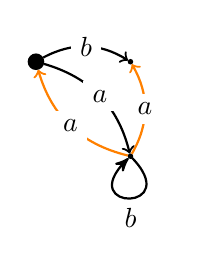
\begin{tikzpicture}[->]
        \GraphInit[vstyle=Simple]
        \SetGraphUnit{1.2}
        \tikzset{VertexStyle/.style={shape=circle, fill=black,
            minimum size=2pt, inner sep=0pt}}
        \tikzset{EdgeStyle/.style={bend left}}

        \begin{scope}[VertexStyle/.append style = {minimum size=6pt}]
          \Vertex{v0}
        \end{scope}
        \EA(v0){c}
        \SO(c){e}

        \Edge[label={$a$}](v0)(e)

        \Edge[label={$b$}](v0)(c)
        \Edge[color=orange, label={$a$}, style={<-}](c)(e)
        \Edge[color=orange, label={$a$}](e)(v0)

        \Loop[label={$b$}, dir=WE, dist=1cm, labelstyle={below}](e)
      \end{tikzpicture}
      \\
      \multicolumn{2}{c}{
        %% Picture 7
        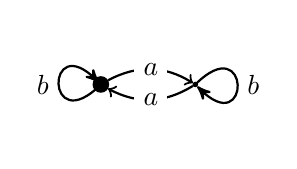
\begin{tikzpicture}[->]
          \GraphInit[vstyle=Simple]
          \SetGraphUnit{1.2}
          \tikzset{VertexStyle/.style={shape=circle, fill=black,
              minimum size=2pt, inner sep=0pt}}
          \tikzset{EdgeStyle/.style={bend left}}

          \begin{scope}[VertexStyle/.append style = {minimum size=6pt}]
            \Vertex{v0}
          \end{scope}
          \EA(v0){e}

          \Edge[label={$a$}](v0)(e)
          \Edge[label={$a$}](e)(v0)

          \Loop[label={$b$}, dir=NO, dist=1cm, labelstyle={left}](v0)
          \Loop[label={$b$}, dir=SO, dist=1cm, labelstyle={right}](e)
        \end{tikzpicture}
      }
    \end{tabular}
  \end{center}
\end{figure}


\begin{figure}
  \caption{\label{fig:tree}%
    Continuing the example from \autoref{fig:example}, the set $Y$ in \autoref{lem:main} is constructed from the minimum spanning tree, shown in bold edges, for the graph produced by Stallings' folding process.
  In this case, $Y = \{b, aba^{-1}, aa\}$.
  The subgroup generated by $Y$ equals the subgroup generated by $U$: the word $aab$ can be produced by the concatenation of $aa$ with $b$, the word $aba^{-1}$ is in both sets, and the word $ba^{-1}ba$ can be expressed as $b \circ (aa)^{-1} \circ aba^{-1} \circ aa$.}
  \begin{center}
    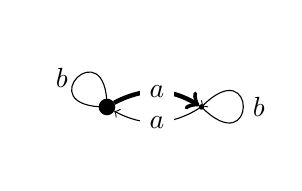
\begin{tikzpicture}[->]
      \GraphInit[vstyle=Simple]
      \SetGraphUnit{1.2}
      \tikzset{VertexStyle/.style={shape=circle, fill=black,
          minimum size=2pt, inner sep=0pt}}
      \tikzset{EdgeStyle/.style={bend left}}

      \begin{scope}[VertexStyle/.append style = {minimum size=6pt}]
        \Vertex{v0}
      \end{scope}
      \EA(v0){e}

      \Edge[label={$a$}, style={ultra thick}](v0)(e)
      \Edge[label={$a$}, style={thin}](e)(v0)

      \Loop[label={$b$}, dir=NOEA, dist=1cm, style={thin}, labelstyle={left}](v0)
      \Loop[label={$b$}, dir=SO, dist=1cm, style={thin}, labelstyle={right}](e)
    \end{tikzpicture}
  \end{center}
\end{figure}

\section{Computing some properties of Stallings' folding process is inherently sequential}
% Foreword

% context (focus on anyone) why now? - current situation, and why the need is so important
According to \autoref{lem:main}, each finitely generated subgroup of a free group corresponds to a directed labeled graph whose language is exactly the generated subgroup.
% need (focus on readers) why you? - why this is relevant to the reader, and why something needed to be done
Since this transformation is efficiently computable we would like to use it to show a reduction to some new computational problems concerning Stallings' folding process.
% task (focus on author) why me? - what was undertaken to address the need
%
%          What to put here???
%
% object (focus on document) why this document - what the document covers
This section proves that determining certain properties of the graph that results from Stallings' folding process is an inherently sequential problem.

% Summary
%
% findings (focus on author) what? - what the work revealed when performing the task
We show that both the problem of determining the additive density of the graph produced by Stallings' folding process and the problem of determining the number of folds performed on parallel edges during the execution of the algorithm are $\P$-complete.
% conclusion (focus on readers) so what? - what the findings mean for the audience
% perspective (focus on anyone) what now? - what should be done next
This is an indication that the algorithm itself is inherently sequential.
In \autoref{sec:pcom}, we use these $\P$-complete problems to show just that.

We first require a basic lemma comparing the number of vertices in a minimal spanning tree to the number of edges in the spanned graph.
The lemma holds for all trees, but we state it for the specific case of minimal spanning trees.
%% This can be found in, for example, Mathematics for Computer Science by
%% Leighton, Meyer, and Lehman.
\begin{lemma}\label{lem:tree}
  Let $G$ be a graph with vertex set $V$ and edge set $E$.
  If $T$ is a minimal spanning tree of $G$ then $|E(T)| = |V(G)| - 1$.
\end{lemma}
\begin{proof}
  This proof is by induction on the number of vertices in the graph.
  Let $T_n$ denote a minimal spanning tree on a graph $G_n$ with $n$ vertices.
  For the base case, consider the graph on one vertex with no edges.
  In this case, the minimal spanning tree $T_1$ is the empty tree, so
  \begin{equation*}
    0 = |E(T_1)| = |V(G)| - 1 = 1 - 1 = 0.
  \end{equation*}
  For the inductive step, suppose that for graphs with $i$ vertices, we have $|E(T_i)| = |V(G_i)| - 1$.
  Consider a minimal spanning tree $T_{i + 1}$ of a graph $G_{i + 1}$ on $i + 1$ vertices.
  Now the subgraph of $T_{i + 1}$ which is just $T_{i + 1}$ with a single leaf removed, call it $T_i$, is a minimal spanning tree of a subgraph of $G_{i + 1}$ which has $i$ vertices, call it $G_i$.
  By the inductive hypothesis, $|E(T_i)| = |V(G_i)| - 1$.
  This implies $|E(T_{i + 1})| = |E(T_i)| + 1 = |V(G_i)| = |V(G_{i + 1})| - 1$, which concludes the proof.
\end{proof}

\begin{theorem}\label{thm:fdpcomplete}
  \FD{} is $\P$-complete, even when the graph is a both a flower graph and a core graph (with respect to the same vertex).
\end{theorem}
\begin{proof}
  By \autoref{thm:finfp}, $F(G)$ is computable in polynomial time.
  Computing the additive density of a graph can be done in linear time, as can comparison with an integer, so \FD{} is in $\P$.

  To show that \FD{} is $\P$-hard, we show a logarithmic space many-one reduction from the $\P$-complete decision problem \FGR{} to \FD{}.
  The reduction is $\langle S, U, k \rangle \mapsto \langle S, G, \mu, k - 1 \rangle$, where $G$ and $\mu$ are the graph and label function guaranteed by \autoref{lem:main}.
  This reduction is computable in logarithmic space by that lemma as well.

  Let $Y$ be the set constructed in \autoref{lem:main} such that the rank of $\gen{U}$ equals $|Y|$.
  In order to show that the reduction is correct, it suffices to show that the additive density of $F(G)$ equals $|Y| - 1$.
  The set $Y$ is defined as
  \begin{equation*}
    Y = \left\{\mu(p_e) \, \middle| \, e \in E(G') \setminus E(T) \right\},
  \end{equation*}
  where $G' = F(G)$ and $T$ is a spanning tree for $G'$.
  Now
  \begin{align*}
    |Y| & = |E(G') \setminus E(T)| & \\
    & = |E(G')| - |E(T)| & \text{ (since } E(T) \subseteq E(G') \text{)} \\
    & = |E(G')| - (|V(G')| - 1) & \text{ (by \autoref{lem:tree})} \\
    & = |E(G')| - |V(G')| + 1 & \\
    & = \delta(G') + 1 & \text{ (by definition of } \delta \text{)}.
  \end{align*}
  With this equality, we conclude the proof by stating that $\gen{U}$ has rank at most $k$ if and only if $\delta(G') + 1 \leq k$.
\end{proof}

\begin{theorem}
  \PFolds{} is $\P$-complete, even when the graph is a both a flower graph and a core graph (with respect to the same vertex).
\end{theorem}
\begin{proof}
  Like for \FD, computing Stallings' folding process and counting the number of folds that occur on a pair of parallel edges places this problem in $\P$.
  We show a logarithmic space many-one reduction from the \FD{} problem on graphs that are both flower graphs and core graphs to \PFolds{}.
  The reduction is $\langle S, G, \mu, k \rangle \mapsto \langle S, G, \mu, \delta(G) - k \rangle$.
  Counting the number of vertices and number of edges in $G$, then performing two subtractions can be performed in logarithmic space.

  It remains to show the correctness of the reduction.
  Each fold in Stallings' folding process decreases the number of edges in the final graph by one.
  Each fold decreases the number of vertices in the final graph by one, unless the fold operates on two parallel edges with the same label (that is, two edges with the same origin, terminus, and label), in which case, the number of vertices remains unchanged.
  (This includes folds of double self-loops.)
  Let $N_F(G)$ be the number of folds when Stallings' folding process is run on input $G$, and let $N^\|_F(G)$ be the number of those folds which are folds of a pair of a parallel edges.
  If $G' = F(G)$, it follows that $|E(G')| = |E(G)| - N_F(G)$ and $|V(G')| = |V(G)| - (N_F(G) - N^\|_F(G))$.
  Hence
  \begin{align*}
    \delta(G') & = |E(G')| - |V(G')| \\
    & = (|E(G)| - N_F(G)) - (|V(G)| - (N_F(G) - N^\|_F(G))) \\
    & = (|E(G)| - |V(G)|) - N_F(G) + N_F(G) - N^\|_F(G) \\
    & = \delta(G) - N^\|_F(G).
  \end{align*}
  Therefore, $\delta(G') \leq k \iff \delta(G) - N^\|_F(G) \leq k \iff N^\|_F(G) \geq \delta(G) - k$.
\end{proof}

\section{Stallings' folding process is inherently sequential}\label{sec:pcom}
% Foreword

% context (focus on anyone) why now? - current situation, and why the need is so important
The previous section shows that computing the additive density of a graph after performing Stallings' folding process is an inherently sequential problem; adding more processors does not provide any substantial speedup.
Since it is easy to compute the additive density of a graph, the hardness of this problem seems to stem from the sequential nature of the folding process: each fold depends on the result of the previous fold.
% need (focus on readers) why you? - why this is relevant to the reader, and why something needed to be done
% ...and task (focus on author) why me? - what was undertaken to address the need
In an effort to formalize this intuition, we would like to prove that Stallings' folding process itself is an inherently sequential algorithm.
% object (focus on document) why this document - what the document covers
This section shows that if there were a highly parallel algorithm that simulates Stallings' folding process, then each polynomial time algorithm could be simulated by a highly parallel algorithm (an outcome widely regarded as unlikely).

% Summary
%
% findings (focus on author) what? - what the work revealed when performing the task
Specifically, we show that Stallings' folding process is $\FP$-complete, and that deciding $\Flow$ is complete for $\P$ under non-adaptive Turing reductions.
% conclusion (focus on readers) so what? - what the findings mean for the audience
This means that computing the function $F$ is among the most difficult of all polynomial time computable functions, and that it should therefore be considered inherently sequential.
% perspective (focus on anyone) what now? - what should be done next
We conjecture that $\Flow$ is complete for $\P$ under logarithmic space many-one reductions (which would mean that $F$ satisfies the definition of ``inherently sequential algorithm'' as given in \autocite[Definition~8.2.2]{ghr95}), but are unable to show it.

\begin{theorem}\label{thm:fpcomplete}
  Stallings' folding process is complete for $\FP$ under logarithmic space single query Turing reductions.
  More generally, Stallings' folding process is $\FP$-complete.
\end{theorem}
\begin{proof}
  As stated in the introduction, Stallings' folding process is in $\FP$.
  In order to show that $F$ is hard for $\P$, it suffices to show a logarithmic space single query Turing reduction from \FD{} to $F$.
  The following logarithmic space Turing machine with access to an oracle for $F$ decides \FD{}.
  On input $\langle S, G, \mu, k \rangle$,
  \begin{itemize}
  \item query $F$ on $\langle S, G, \mu \rangle$ to get graph $G'$ and label function $\mu'$,
  \item compute $|Y|$ as in \autoref{lem:main},
  \item accept if and only if $|Y| \geq k$.
  \end{itemize}
  Since the rank of $\gen{U}$ equals $|Y|$, the correctness of the reduction follows.
\end{proof}

We can use the fact that $F$ is $\FP$-complete to show that $\Flow$ is complete for $\P$ under logarithmic space non-adaptive Turing reductions.
The completeness of $\Flow$ follows from the following two lemmas.
The first shows that logarithmic space nonadaptive Turing reductions compose.
The second provides a method for transforming an $\FP$-complete function into a language that is complete for $\P$ under logarithmic space nonadaptive Turing reductions.

\begin{lemma}\label{lem:compose}
  Logarithmic space nonadaptive Turing reductions compose.
\end{lemma}
\begin{proof}
  Let $A$, $B$, and $C$ be arbitrary languages.
  Suppose there are functions $g$ and $h$ in $\FL$ and logarithmic space Turing machine $M$ and $N$ such that $x \in A$ if and only if $M(x, B(y_1), \dotsc, B(y_s))$ accepts and $y \in B$ if and only if $N(y, C(z_1), \dotsc, C(z_t))$ accepts, where $g(x) = (y_1, \dotsc, y_s)$ and $h(y) = (z_1, \dotsc, z_t)$.

  Let $g(x)_i$ denote the $i$th string in the $s$-tuple output by $g(x)$.
  Define function $h'$ by $h'(x) = h(g(x)_1) \circ \dotsb \circ h(g(x)_s)$ for all strings $x$, where $\circ$ denotes concatenation of tuples.
  The function $h'$ is in $\FL$ because $\FL$ functions compose.
  Define Turing machine $M'$ as follows.
  On input string $x$ and oracle answers $C(z_{1, 1}), \dotsc, C(z_{1, t_1}), \dotsc, C(z_{s, 1}), \dotsc, C(z_{s, t_s}))$,
  \begin{itemize}
  \item simulate $g(x)$ to yield $(y_1, \dotsc, y_s)$,
  \item for each $y_i$, simulate $N(y_i, C(z_{i, 1}), \dotsc, C(z_{i, t_i}))$ to yield output bit $b_i$,
  \item simulate $M(x, b_1, \dotsc, b_s)$.
  \end{itemize}
  The Turing machine $M'$ runs in logarithmic space because it is essentially computing the composition of three logarithmic space computable functions: $g$, $N$, and $M$.
  We claim that $h'$ and $M'$ together constitute the reduction from $A$ to $C$.

  By hypothesis $x \in A$ if and only if $M(x, B(y_1), \dotsc, B(y_s))$ accepts.
  Also by hypothesis, for each $y_i$, we have $y_i \in B$ if and only if $N(y_i, C(z_{i, 1}), \dotsc, C(z_{i, t_i}))$ accepts.
  Thus $x \in A$ if and only if
  \begin{equation}\label{eq:m}
    M(x, N(y_1, C(z_{1, 1}), \dotsc, C(z_{1, t_1})), \dotsc, N(y_s, C(z_{s, 1}), \dotsc, C(z_{s, t_s})))
  \end{equation}
  accepts.
  By construction $M'(x, C(z_{1, 1}), \dotsc, C(z_{s, t_s}))$ computes exactly the same function as the machine in \eqref{eq:m}, so the reduction is correct.
\end{proof}

\begin{lemma}\label{lem:nonadaptive}
  Suppose $f$ is a function and define $B_f$ by
  \begin{equation*}
    B_f = \{ \langle x, i, b \rangle | \text{the } i \text{th bit of } f(x) \text{ is } b \}.
  \end{equation*}
  If $f$ is complete for $\FP$ under logarithmic space single query Turing reductions, then $B_f$ is complete for $\P$ under logarithmic space nonadaptive Turing reductions.
\end{lemma}
\begin{proof}
  Let $L$ be an arbitrary language in $\P$.
  We know that there is a logarithmic space Turing machine $M$ that decides $L$ while making a single query to oracle $f$.
  Assume without loss of generality that the machine makes its query at the beginning of the computation (this can be done by doing any preprocessing required by $M$ within the reduction).
  Construct machine $M'$ to decide $L$ with oracle access to $B_f$.
  The machine $M'$ simulates $M$, but replaces its single query $x$ with $p(|x|)$ queries of the form $\langle x, i, 1 \rangle$, one for each $i$ in $\{1, \dotsc, p(|x|) \}$, where $p$ is the polynomial that bounds the running time of $f$.
  Whenever the oracle responds to query $\langle x, i, 1 \rangle$ with a $1$, we know the $i$th bit of $f(x)$ is $1$, and whenever the oracle responds with $0$, we know the $i$th bit of $f(x)$ is $0$.
  In this way, $M'$ reconstructs $f(x)$, then proceeds with the computation of $M$.
  Thus $M'$ is a correct logarithmic space Turing machine that decides $L$ with nonadaptive oracle access to $B_f$.
\end{proof}

\begin{theorem}
  \Flow{} is complete for $\P$ under logarithmic space non-adaptive Turing reductions, even when the input to $F$ is a flower graph and a core graph (with respect to the same vertex).
\end{theorem}
\begin{proof}
  \Flow{} is in $\P$ because Stallings' folding process is computable in polynomial time, and checking individual bits of the computation history can be done in polynomial time as well.

  By \autoref{thm:fpcomplete} and \autoref{lem:nonadaptive}, $B_F$ is complete under logarithmic space nonadaptive Turing reductions.
  It suffices to show a logarithmic space many-one reduction from $B_F$ to \Flow{}, since a many-one reduction implies a nonadaptive Turing reduction, and logarithmic space nonadaptive Turing reductions compose (\autoref{lem:compose}).
  The reduction is $\langle \langle S, G, \mu \rangle, i, b \rangle \mapsto \langle \langle S, G, \mu \rangle, i', b\rangle$, where $i'$ is the index of the $i$th bit of the last binary string written during the computation of $F$ (assuming without loss of generality that $F$ writes its output to memory immediately before halting).
  Bit $i'$ in the flow function is exactly the same as the $i$th bit of $F(S, G, \mu)$, so the reduction is correct.
\end{proof}

The preceding theorem is weaker than we would like.
Our goal is to show that Stallings' folding process is inherently sequential.
In order to do that, we would need to prove that \Flow{} is complete for $\P$ under logarithmic space \emph{many-one} reductions.
We believe this to be true but are unable to prove it.

\begin{conjecture}
  Stallings' folding process is inherently sequential (that is, \Flow{} is complete for $\P$ under logarithmic space many-one reductions).
\end{conjecture}

\printbibliography

\end{document}
